\section{Taxonomies of Usage Management Overlay}
A clear taxonomic organization of potential steps in approaching finer grained policy based usage management helps in describing the difficulties inherent in developing potential solutions as well as aiding in planning system evolution over time. Here, we have five distinct types of integrated policy-centric usage management systems, as shown in Table \ref{table:model:taxonomy}.  Of these five, only the first two levels are represented in current system model.

\begin{table*}[tp] %
\centering %
\begin{tabular}{clcc}
\toprule %
$ Name$ 	& $Description$ \\\toprule %
$\phi$ 		& The initial level of this taxonomy, $\phi$ classified systems \\
 			& have a single guard without policy-based control \\\midrule
$\alpha$	& $\alpha$ classified systems have a single guard by have begun \\
			& to integrate policy-based control \\\midrule
$\beta$		& Systems that have begun to integrate policy-based control with \\
			& router elements are in the $\beta$ category \\\midrule
$\gamma$	& Systems that have integrated policy-based control with routing \\
			& and computational elements \\\midrule
$\delta$	& Continuous policy-based control with \textit{smart licensed} artifacts \\\bottomrule
\end{tabular}
\caption{Proposed Usage Management Taxonomy}
\label{table:model:taxonomy}
\end{table*}

In this taxonomy, it is not required that systems pass through lower levels to reach higher ones.  This taxonomy represents a continuum of integration of usage management controls.  Systems can very well be designed to fit into higher taxonomic categories without addressing lower categories.  That said however, many of the supporting infrastructural services, like identification management or logging and tracing systems, are common between multiple levels.

The taxonomy itself starts with the current state, integrating policy evaluation systems into the network fabric gradually, moving away from filters, then by adding policy evaluation into the routing fabric, then the computational nodes, and finally by incorporating evaluation directly into content.

\subsection{$\phi$-level Overlay Systems}
The $\phi$ classification consists of systems like the initial NSA and BAH notional models.  These systems consist of two distinct domains, separated by a filter-centric single guard.  The initial NSA system model is clearly of this type, separating two domains with a guard using filter chains.  The BAH model is also of this type, using a Filter Segment to evaluate data packages transmitted between interface segments attached to specific domains.

\begin{figure}[!t]
\centering
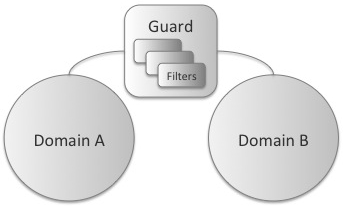
\includegraphics[width=3in]{model-phi-crop}
\caption{Taxonomy ($\phi$)}
\label{fig:model:taxonomy-phi}
\end{figure}

Generally one of the domains supports more sensitive information than the other, but that is not always the case.  In the models we have examined this has certainly been true, but classified information for example  is commonly stored in \textit{compartments} which are separated by clear \textit{need-to-know} policies enforced by access lists and classification guides.  These kinds of compartments contain information at similar levels of classification, but contain distinct informational elements that should not be combined.

In these kinds of systems, specific rules regarding information transfer and domain characterization are tightly bound to individual filter implementations.  They are based on \textit{a priori} knowledge of the domains the guard connects, and therefore are tightly coupled to the domains they connect.  Furthermore, the filter elements are standalone within the system, in this classification, not availing themselves of external resources.  Rather, they examining information transiting through the filter based purely on the content of that information.

\subsection{$\alpha$-level Overlay Systems}
The $\alpha$ overlay classification contains systems that have begun to integrate policy-centric usage management.

Both policies and contexts are dynamically delivered to the system.

The dynamic delivery of context and policies allows these kinds of systems more flexibility with policy evaluation.

The $\alpha$ category begins to integrate policy-centric management rather than using strict content filtering.

\begin{figure}[!t]
\centering
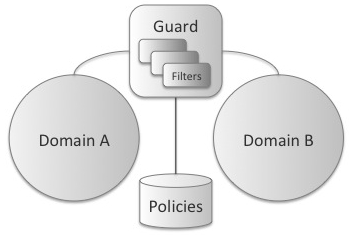
\includegraphics[width=3in]{model-alpha-crop}
\caption{Taxonomy ($\alpha$)}
\label{fig:model:taxonomy-alpha}
\end{figure}

Here, we again have at least two domains, Domain A and Domain B, though we could potentially have more.  $\phi$ type systems require domain specific information to be tightly coupled to the filter implementations.  Separating the permissions, obligations, and other constraints from the filters and incorporating them into a specific separate policy entity frees the Guard from this coupling and provides additional flexibility to the system.

The guard can continue to use filters to process data.  These filters however are now more generic and decoupled from the specific domains it manages.  The choice of using a specific filtering model rather than some other kind of construct is a design detail level to implementers.  That said however, individual filters will be remarkably different and still need to understand the ontologies over which specific licenses are defined.

The policy repository is key to the implementation and differentiation of this taxonomy category.  This repository can be implemented as a separate repository keyed into via a data artifact's unique URI, for example.  It could also represent a policy sent in tandem with a data artifact in a data package.

The policy repository may be implemented as some kind of external service, and as such, represents the first such external service explicitly used in this taxonomy.  Other external services may well exist and be used to adjudicate information transfer decisions as well.

\subsection{$\beta$-level Overlay Systems}
The $\beta$ taxonomic category begins to integrate policy-centric processing with router elements in a given network.  While this work is centered on using overlay technology to illustrate and implement these concepts, it is important to note that this kind of distributed policy-centric processing could very well be distributed into the physical routing fabric of a given network as well by extending Software Defined Networking systems like OpenFlow \cite{proposal:openflow}.

\begin{figure}[!t]
\centering
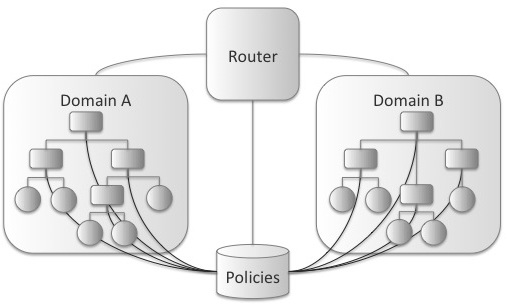
\includegraphics[width=3in]{model-beta-crop}
\caption{Taxonomy ($\beta$)}
\label{fig:model:taxonomy-beta}
\end{figure}

In this model we can also host multiple domains as a result of flexible policy-based content examination.  Each domain hosts a network of some kind, though that hosted network could very well be a degenerate network of a single system.  Each network hosted in a domain is hierarchical, with specific computational nodes embodied by workstations, tablet computers or mobile devices, and routing points embodied by routers or switches of some kind.

Policy evaluation in this model has begun to penetrate into the routing elements of the specific domain networks.  Here, note that we have started to penetrate into the routing fabric of the network by doing content evaluation at router points.  Content-based switching networks have been successful in other domains, and such techniques can be used here to provide policy evaluation capabilities.  

Certain types of traffic are easier to evaluate than others however.  For example, HTTP requests and responses are easier to examine that TCP packets.  When examining TCP packets, systems generally require additional context to select an appropriate packet window (e.g. the number of packets cached for examination).  HTTP traffic does not usually require this kind of flexibility.

This migration of policy evaluation into the routing fabric provides for enhanced data security and better network management, especially if part of a network is compromised.  Now that policy decisions can be made at the router level in a given network, we are starting to have network security in depth rather than simple perimeter protection.  This not only provides the ability for additional information protection, but also allows for different compartments holding information at different need-to-know levels to be created ad-hoc under different routing segments.  In cases of network compromise, this kind of dynamic policy enforcement can also allow for quick node excision as well.

\subsection{$\gamma$-level Overlay Systems}
The $\gamma$ compartment has integrated policy evaluation with compute and routing nodes.  Here, policies can be evaluated against content at all network levels --- nodes emitting requests, nodes fielding requests, and all routing elements in between.

\begin{figure}[!t]
\centering
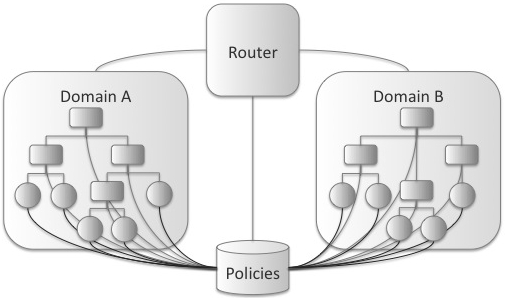
\includegraphics[width=3in]{model-gamma-crop}
\caption{Taxonomy ($\gamma$)}
\label{fig:model:taxonomy-gamma}
\end{figure}

We see that the policy repository is supplying services to all computational elements in both domains.  This gives us increased granularity with respect to data compartmentalization by integrating information security into each network element.  At this point, the network can create compartments of single nodes, while previously in $\beta$ level systems compartments could only be created under specific routing elements.  At this level, we can also provide services revoking data access based on policy evaluation decisions when needed.

Furthermore, individual node exclusion is possible as well. $\beta$ classified systems could excise network elements under specific routers by dynamic policy application.  Now, we can apply the same functionality to individual compute nodes.  For example, if a networked device like a smart phone is compromised, that device can be removed from access quickly or used to feed mis-information to adversaries.

\section{Taxonomic Analysis}
The various levels of the taxonomy vary primarily with respect to the inclusion of policy-based usage management and overlay structure.  $\phi$ type systems are not structured with overlay use in mind, nor do they use policy-centric management.  Conversely, $\gamma$ type systems are both purely policy oriented and completely overlay structured.

As systems move through the various levels of the taxonomy they gradually move from one side of the spectrum to another.  Overlay structures, hierarchical or otherwise, gradually migrate into the network begining with $\beta$ systems.  Policy orientation is injected into the architectures starting with $\alpha$ systems and moving into the network fabric in parallel with overlay inclusion.

\subsection{Policy-centricity}
In these systems policy based management supplies distinct advantages over filter-centric information control.  This kind of policy-centric usage management is more content specific than filters, more flexible, is more expressive, allows for better content traceability, and finally provides a clear separation of concerns not shown by filter systems.

\subsubsection*{Content Specific}
Filters, in filter-based systems, are not coupled to the content passing through the system.  Rather, they are usually tied to the characteristics of attached networks.  For some filters, that is not problematic.  Malware filters, for example, are very general and do not need to have an understanding of filtered content and are not sensitive to that content at all, though they can be very sensitive to specific context.  This limitation does however prohibit filters from doing anything content specific.  Due to their deployment limitations, in that they are deployed to such a system via a process distinct from processing content, they are unable to use presented content or current dynamic context to influence information processing decisions.

Consider content $c$ impacted by a dynamic context $d$ where $d$ is defined in terms of the content itself, the person or system requesting that content, and the environment in which that request is made.  Here, only under certain specific environmental conditions is that requesting agent allowed access to the requested content.  Ergo, the decision with regard to pass the content to the requester is based upon characteristics of the content related to dynamic changes within the environment.  A filter-centric solution like that contained within the $\phi$ level of the taxonomy is unable to change filter rules based on changes like new content or environmental alteration.  A policy-based system, on the other hand, is able to express the content specific policy easily for more dynamic evaluation.

For example, if $c$ contains information that can only be accessed for a specific time period, a static filter simply cannot determine that the information in $c$ is no longer appropriate for dissemination after that time period ends.  That kind of evaluation requires meta-data associated with $c$ that specifically describes these time bounds and a dynamic contextual evaluator able to determine when that window of access has closed.  That meta-data in this case is a policy.

\subsubsection*{Flexibility}
Policy-centric systems are more flexible than filter-based counterparts.  In a filter-based solution, the type of content that can be evaluated is tightly coupled to the filters installed.  If a given piece of content is new to a given filter-centric solution, that content cannot be appropriately examined and must be submitted for human review.  A policy-based system is designed to be more general.  Based upon a common ontology ~\cite{JaHeLa:10}, the evaluation system can be very general with respect to it's evaluation of a given policy.  A general policy engine can handle a great variety of different content as long as the policies associated with that content correspond to known domain ontologies.  This generality leads to a greater amount of flexibility with respect to what can be expressed in a specific policy, and leads to a more flexible maintainable system.

A filter is going to have a specific responsibility, like redacting sensitive words from a document, for instance.  In order for that filter to redact those sensitive words, it must have access to some kind of list of what those sensitive words are.  Remember, $\phi$ level systems use static filters, so that filter can only be updated when the filter itself is updated.  Now a policy-centric system on the other hand can have a policy associating sensitivity with various areas of content in a specific document.  In this case, all the system must do is understand the sensitivity described in the policy associated with the content, and can then redact that content if needed.  The ontology describing the areas of sensitivity will change more slowly that the possible content itself, leading to a more flexible maintainable system.

This is of course a simple example solvable by creating a dynamic list; the key point of the above example is that the specificity of the filters requires additional complexity in the filter system itself.  The generality of the policy-centric system allows the complexity to be more clearly expressed and contained within the policy file.

\subsubsection*{Expressiveness}
While filters can process content at specific perimeter points, it's lack of reach into a given network fabric limits the power a given filter can actually have over transmitted content.  A policy associated with content, when transmitted with content, can reference much more than the semantics of the protected content.  That policy can describe specifically, in detail, how that content can be used.  Filters simply cannot exercise that level of control.

Assume a distributed system with multiple filter points.  In this kind of system, information distribution can be controlled via deployed filters at a relatively fine level of granularity.  This kind of distribution control cannot influence the use of protected content however --- one that content is distributed, possessors are accorded full access.

Policy enabled systems are not limited in this way.  Policies, when coupled with policy evaluation tools, can exercise control not only over distribution and routing, but also over use of distributed content at endpoints.

\subsubsection*{Content Traceability}

\subsubsection*{Separation of Concerns}
Section

These advantages accrue in usage management systems as policy capabilities are propagated through the network fabric.

\subsection{Overlay Structure}
Overlay structure integration exhibits clear advantages over single point perimeter systems as well.  Specifically, overlay systems are more partition-able than perimeter solutions, enables content throttling, provides capabilities for dynamic content control, and allows content to be more traceable.

\subsubsection*{Partition-ability}

\subsubsection*{Content Throttling}

\subsubsection*{Dynamic Content Control}

\subsubsection*{Traceability}
Section

The strengths of overlay systems over single perimeter points gradually increase as overlay structures increasingly permeate any given system.